\documentclass[12pt]{article}
\usepackage[margin=1in]{geometry}
\usepackage{amsmath,amssymb,mathtools}
\usepackage{enumitem}
\usepackage{bm}
\usepackage{hyperref}
\usepackage{fancyhdr}
\usepackage{draftwatermark}
\usepackage{xcolor}
\usepackage{pgfplots}
\usepackage{titlesec}
\pgfplotsset{compat=newest}

%------------- TITLE AND METADATA -------------
\newcommand{\CourseCode}{HE2002 }
\newcommand{\CourseName}{Macroeconomics II}
\newcommand{\DocType}{Tutorial 7}

\title{
\CourseCode \CourseName \\[0.3em]
\large \DocType
}
\author{
  Academic Year 2025/2026, Semester 2 \\[0.25em]
  \textit{Quantitative Research Society @NTU}
}
\date{\today}

%------------- HEADER & FOOTER (for page 2 onward) -------------
\fancypagestyle{main}{
  \fancyhf{}
  \fancyhead[L]{\CourseCode \CourseName \ --\ \DocType}
  \fancyhead[R]{\href{https://qrsntu.org}{QRS@NTU}}
  \fancyfoot[C]{\thepage}
  \renewcommand{\headrulewidth}{0.4pt}
  \renewcommand{\footrulewidth}{0pt}
}

%------------- SIMPLE FOOTER (page 1 only) -------------
\fancypagestyle{plainfirst}{
  \fancyhf{}
  \renewcommand{\headrulewidth}{0pt}
  \renewcommand{\footrulewidth}{0pt}
  \fancyfoot[C]{\scriptsize\textcolor{gray}{\textit{For academic reference only. This document is provided for educational purposes and does not constitute an official question paper, answer key, or any formally authorised academic material. Its content is not guaranteed to be complete or accurate.}}}
}

%------------- WATERMARK -------------
\SetWatermarkText{Unofficial — QRS@NTU — qrsntu.org}
\SetWatermarkScale{1}
\SetWatermarkLightness{0.99}

%------------- SHORTCUTS -------------
\newcommand{\R}{\mathbb{R}}
\newcommand{\Rp}{\mathbb{R}_+}
\newcommand{\E}{\mathbb{E}}
\newcommand{\Var}{\mathrm{Var}}
\newcommand{\dotp}{\cdot}

%------------- STYLE -------------
\setlist[enumerate]{itemsep=0.32em, topsep=0.32em}
\setlist[itemize]{itemsep=0.22em, topsep=0.22em}

\titleformat{\subsubsection}[block]
{\normalfont\large\bfseries}
{}
{0pt}
{}

\titleformat{\paragraph}[block]
{\normalfont\normalsize\bfseries}
{}
{0pt}
{}

\titlespacing*{\paragraph}
{0pt}
{1.2ex}
{0.6ex}

\setcounter{secnumdepth}{0}
\setcounter{tocdepth}{4}

\begin{document}

\maketitle
\thispagestyle{plainfirst}
\pagestyle{main}
\bigskip

%====================================================
% OVERVIEW
%====================================================
\begin{center}
  \rule{0.8\textwidth}{0.4pt}\\[4pt]
  \textbf{Overview}\\[2pt]
  \rule{0.8\textwidth}{0.4pt}
\end{center}

\noindent
This tutorial covers:
\begin{itemize}[leftmargin=*]
  \item the Phillips curve under different assumptions about inflation expectations;
  \item the natural rate of unemployment and the inflationary consequences of holding unemployment below it;
  \item the distinction between anchored and adaptive expectations;
  \item the role of wage indexation in altering inflation dynamics;
  \item comparative inflation paths with and without indexed labour contracts;
  \item graphical and algebraic interpretation of how unemployment affects inflation.
\end{itemize}

\bigskip

\newpage
\tableofcontents

\newpage
%====================================================
% QUESTION 1
%====================================================
\section{Question 1: Mutations of the Phillips Curve}

\noindent
Chapter 8, Q5. Mutations of the Phillips curve

\subsection{Problem}
Suppose that the Phillips curve is given by
\[
\pi_t=\pi_t^e+0.1-2u_t
\]
and expected inflation is given by
\[
\pi_t^e=(1-\theta)\bar{\pi}+\theta\pi_{t-1}
\]
and suppose that \(\theta\) is initially equal to 0, and that \(\bar{\pi}\) is given and does not change. It could be zero or any positive value.

Suppose that the rate of unemployment is initially equal to the natural rate. In year \(t\), the authorities decide to bring the unemployment rate down to 3\% and hold it there forever.
\begin{enumerate}[label=(\alph*)]
    \item Determine the rate of inflation in periods \(t+1\), \(t+2\), \(t+3\), \(t+4\), \(t+5\). How does \(\bar{\pi}\) compare to \(\pi\)?
    \item Do you believe the answer given in part a? Why or why not? \emph{(Hint: Think about how people are more likely to form expectations of inflation.)}
\end{enumerate}

Now suppose that in year \(t+6\), \(\theta\) increases from 0 to 1. Suppose that the government is still determined to keep \(u\) at 3\% forever.
\begin{enumerate}[label=(\alph*),start=3]
    \item Why might \(\theta\) increase in this way?
    \item What will the inflation rate be in years \(t+6\), \(t+7\), and \(t+8\)?
    \item What happens to inflation when \(\theta=1\) and unemployment is kept below the natural rate of unemployment?
    \item What happens to inflation when \(\theta=1\) and unemployment is kept at the natural rate of unemployment?
\end{enumerate}

\newpage
\subsection{Solution}

\subsubsection{Method 1: Direct recursive substitution from the expectations equation}
We first determine the natural rate of unemployment. By definition, at the natural rate inflation equals expected inflation, so
\[
\pi_t=\pi_t^e
\quad\Longrightarrow\quad
0.1-2u_n=0.
\]
Hence
\[
2u_n=0.1
\quad\Longrightarrow\quad
u_n=0.05.
\]
Therefore,
\[
\boxed{u_n=5\%.}
\]

Because unemployment is initially equal to the natural rate and \(\theta=0\), expected inflation is initially
\[
\pi_s^e=(1-0)\bar{\pi}+0\cdot \pi_{s-1}=\bar{\pi},
\]
so before the policy change actual inflation is also equal to \(\bar{\pi}\).

\begin{enumerate}[label=(\alph*)]
    \item
    From year \(t\) onward the government keeps unemployment at
    \[
    u=3\%=0.03.
    \]
    While \(\theta=0\), expected inflation remains fixed at
    \[
    \pi_s^e=\bar{\pi}
    \]
    in every such year. Hence for any year \(s=t,t+1,\dots,t+5\),
    \[
    \pi_s=\pi_s^e+0.1-2u_s
    =\bar{\pi}+0.1-2(0.03)
    =\bar{\pi}+0.1-0.06
    =\bar{\pi}+0.04.
    \]
    Therefore
    \[
    \pi_{t+1}=\pi_{t+2}=\pi_{t+3}=\pi_{t+4}=\pi_{t+5}=\bar{\pi}+0.04.
    \]
    So the requested inflation path is
    \[
    \boxed{\pi_{t+1}=\pi_{t+2}=\pi_{t+3}=\pi_{t+4}=\pi_{t+5}=\bar{\pi}+0.04.}
    \]

    Thus actual inflation is higher than \(\bar{\pi}\) by \(0.04\), that is, by 4 percentage points:
    \[
    \boxed{\pi=\bar{\pi}+0.04 \quad\Longrightarrow\quad \bar{\pi}<\pi.}
    \]

    \item
    Taken literally, part (a) says that inflation jumps up by 4 percentage points and then stays there forever, despite unemployment remaining below the natural rate forever. This is not very believable.

    The reason is that when inflation is persistently above the previously expected level, people are unlikely to continue forming expectations using a fixed anchor \(\bar{\pi}\) only. They will begin to look at recent actual inflation. Workers, firms, and wage setters learn from the inflation they observe. Hence expected inflation should gradually move upward, and once that happens, actual inflation should continue rising if unemployment remains below the natural rate.

    Therefore the answer in part (a) is mechanically correct under the assumption \(\theta=0\), but economically it is not very plausible for a long-lasting regime:
    \[
    \boxed{\text{The answer in part (a) is algebraically correct under }\theta=0,\text{ but not very realistic.}}
    \]

    \item
    A rise in \(\theta\) from 0 to 1 means that expected inflation moves from being based entirely on the fixed anchor \(\bar{\pi}\) to being based entirely on last period's actual inflation:
    \[
    \pi_t^e=(1-\theta)\bar{\pi}+\theta\pi_{t-1}.
    \]
    When inflation has been persistently positive and salient, it becomes natural for workers and firms to use recent inflation as the benchmark for wage bargains and price setting. This may happen because:
    \begin{itemize}[leftmargin=*]
        \item inflation has become more visible and persistent;
        \item wage setters and price setters learn from past inflation outcomes;
        \item contracts and bargaining norms become more backward-looking;
        \item the economy becomes less anchored to a fixed long-run inflation norm.
    \end{itemize}
    Hence \(\theta\) may increase because expectations formation becomes adaptive:
    \[
    \boxed{\theta \text{ may rise because people begin using actual past inflation to form expectations.}}
    \]

    \item
    Up to year \(t+5\), we found that
    \[
    \pi_{t+5}=\bar{\pi}+0.04.
    \]
    In year \(t+6\), \(\theta=1\), so expected inflation becomes
    \[
    \pi_{t+6}^e=\pi_{t+5}=\bar{\pi}+0.04.
    \]
    Since unemployment is still \(0.03\),
    \[
    \pi_{t+6}=\pi_{t+6}^e+0.1-2(0.03)
    =(\bar{\pi}+0.04)+0.04
    =\bar{\pi}+0.08.
    \]
    Next,
    \[
    \pi_{t+7}^e=\pi_{t+6}=\bar{\pi}+0.08,
    \]
    so
    \[
    \pi_{t+7}=\pi_{t+7}^e+0.04
    =\bar{\pi}+0.12.
    \]
    Similarly,
    \[
    \pi_{t+8}^e=\pi_{t+7}=\bar{\pi}+0.12,
    \]
    so
    \[
    \pi_{t+8}=\pi_{t+8}^e+0.04
    =\bar{\pi}+0.16.
    \]

    Therefore,
    \[
    \boxed{\pi_{t+6}=\bar{\pi}+0.08,\qquad \pi_{t+7}=\bar{\pi}+0.12,\qquad \pi_{t+8}=\bar{\pi}+0.16.}
    \]

    \item
    When \(\theta=1\), expected inflation is
    \[
    \pi_t^e=\pi_{t-1}.
    \]
    Therefore the Phillips curve becomes
    \[
    \pi_t=\pi_{t-1}+0.1-2u_t.
    \]
    If unemployment is kept below the natural rate, then \(u_t<u_n=0.05\), so
    \[
    0.1-2u_t>0.
    \]
    Hence
    \[
    \pi_t-\pi_{t-1}>0
    \]
    in every period. Inflation therefore rises continuously over time.

    So when \(\theta=1\) and unemployment is kept below the natural rate, inflation accelerates:
    \[
    \boxed{\text{Inflation keeps increasing over time.}}
    \]

    \item
    If unemployment is kept at the natural rate, \(u_t=u_n=0.05\), then
    \[
    0.1-2u_t=0.1-2(0.05)=0.
    \]
    Hence, when \(\theta=1\),
    \[
    \pi_t=\pi_{t-1}.
    \]
    So inflation no longer rises or falls; it stays constant at whatever level it has already reached.

    Therefore,
    \[
    \boxed{\text{Inflation remains constant when }u=u_n\text{ and }\theta=1.}
    \]
\end{enumerate}

\newpage
\subsubsection{Method 2: Natural-rate reformulation and accelerationist form}
We rewrite the Phillips curve around the natural rate. Since
\[
0.1-2u_t=-2(u_t-0.05),
\]
the equation
\[
\pi_t=\pi_t^e+0.1-2u_t
\]
can be written as
\[
\pi_t=\pi_t^e-2(u_t-u_n),
\qquad
u_n=0.05.
\]
Thus
\[
\boxed{\pi_t=\pi_t^e-2(u_t-u_n),\qquad u_n=5\%.}
\]

\begin{enumerate}[label=(\alph*)]
    \item
    While \(\theta=0\), expected inflation is fixed at
    \[
    \pi_t^e=\bar{\pi}.
    \]
    The government sets
    \[
    u_t=0.03,
    \qquad
    u_t-u_n=0.03-0.05=-0.02.
    \]
    Hence
    \[
    \pi_t=\bar{\pi}-2(-0.02)=\bar{\pi}+0.04.
    \]
    Since this is the same in every year up to \(t+5\),
    \[
    \boxed{\pi_{t+1}=\pi_{t+2}=\pi_{t+3}=\pi_{t+4}=\pi_{t+5}=\bar{\pi}+0.04.}
    \]

    The comparison is immediate:
    \[
    \boxed{\pi-\bar{\pi}=0.04>0.}
    \]

    \item
    Under \(\theta=0\), inflation does not feed into future expected inflation. This is what prevents inflation from continuing to rise in part (a). In reality, persistent inflation normally affects expectations, so a permanently lower unemployment rate should not merely cause a one-time increase in inflation; it should generate ongoing inflation pressure once expectations become adaptive. Hence the answer in part (a) is best viewed as a special-case outcome tied to an implausibly rigid expectations rule.

    Therefore,
    \begin{center}
    \fbox{\parbox{0.9\linewidth}{\centering
    Part (a) is a special-case result that is not very plausible in a persistent inflationary environment.
    }}
    \end{center}

    \item
    The parameter \(\theta\) measures the weight placed on past actual inflation in expectation formation. A move from \(\theta=0\) to \(\theta=1\) means the economy moves from fully anchored expectations to fully adaptive expectations. This may occur when inflation has lasted long enough that agents no longer trust a fixed benchmark \(\bar{\pi}\) and instead extrapolate from observed inflation.

    Thus,
    \[
    \boxed{\theta \uparrow \text{ because expectation formation becomes more backward-looking and adaptive.}}
    \]

    \item
    When \(\theta=1\),
    \[
    \pi_t^e=\pi_{t-1},
    \]
    so the Phillips curve becomes the accelerationist form
    \[
    \pi_t-\pi_{t-1}=-2(u_t-u_n).
    \]
    Since \(u_t=0.03\) and \(u_n=0.05\),
    \[
    \pi_t-\pi_{t-1}=-2(-0.02)=0.04.
    \]
    Therefore inflation increases by 4 percentage points each year after expectations become adaptive.

    Using \(\pi_{t+5}=\bar{\pi}+0.04\),
    \[
    \pi_{t+6}=\pi_{t+5}+0.04=\bar{\pi}+0.08,
    \]
    \[
    \pi_{t+7}=\pi_{t+6}+0.04=\bar{\pi}+0.12,
    \]
    \[
    \pi_{t+8}=\pi_{t+7}+0.04=\bar{\pi}+0.16.
    \]

    Hence,
    \[
    \boxed{\pi_{t+6}=\bar{\pi}+0.08,\qquad \pi_{t+7}=\bar{\pi}+0.12,\qquad \pi_{t+8}=\bar{\pi}+0.16.}
    \]

    \item
    If \(\theta=1\) and \(u_t<u_n\), then
    \[
    \pi_t-\pi_{t-1}=-2(u_t-u_n)>0.
    \]
    Therefore inflation rises period after period without settling down:
    \[
    \boxed{\text{Inflation accelerates whenever }u_t<u_n\text{ and }\theta=1.}
    \]

    \item
    If \(\theta=1\) and \(u_t=u_n\), then
    \[
    \pi_t-\pi_{t-1}=-2(u_n-u_n)=0.
    \]
    Therefore,
    \[
    \boxed{\pi_t=\pi_{t-1},}
    \]
    so inflation stays constant:
    \[
    \boxed{\text{Inflation is stable when unemployment is kept at the natural rate.}}
    \]
\end{enumerate}

\begin{center}
\[
\begin{array}{c|cccccccc}
\text{Year} & t & t+1 & t+2 & t+3 & t+4 & t+5 & t+6 & t+7 \\ \hline
\theta=0 & \bar{\pi}+0.04 & \bar{\pi}+0.04 & \bar{\pi}+0.04 & \bar{\pi}+0.04 & \bar{\pi}+0.04 & \bar{\pi}+0.04 & - & - \\
\theta=1 & - & - & - & - & - & \bar{\pi}+0.04 & \bar{\pi}+0.08 & \bar{\pi}+0.12
\end{array}
\]
\end{center}

\newpage
%====================================================
% QUESTION 2
%====================================================
\section{Question 2: The Macroeconomic Effects of the Indexation of Wages}

\noindent
Chapter 8, Q6. The macroeconomic effects of the indexation of wages

\subsection{Problem}
Suppose that the Phillips curve is given by
\begin{equation}
\pi_t-\pi_t^e=0.1-2u_t \tag{1}
\end{equation}
where
\begin{equation}
\pi_t^e=\pi_{t-1} \tag{2}
\end{equation}

Suppose that inflation in year \(t-1\) is zero. (There is a typo in the textbook.) In year \(t\), the central bank decides to keep the unemployment rate at 4\% forever.
\begin{enumerate}[label=(\alph*)]
    \item Compute the rate of inflation for years \(t\), \(t+1\), \(t+2\) and \(t+3\).
\end{enumerate}

Now suppose that half the workers (50\%) have indexed labor contracts. It is introduced in Section 8.4 in the textbook:

When the inflation rate becomes high, the terms of wage agreements tend to change with the level of inflation. Wage indexation is a provision that automatically increases wages in line with inflation. Suppose \(\lambda\) a proportion of labor contracts that is indexed, so nominal wages move one-for-one with changes in the actual price level, the Phillips curve becomes:
\begin{equation}
\pi_t=\left[\lambda\pi_t+(1-\lambda)\pi_{t-1}\right]-\alpha(u_t-u_n) \tag{3}
\end{equation}
When \(\lambda>0\), equation (3) becomes:
\begin{equation}
\pi_t-\pi_{t-1}=-\frac{\alpha}{1-\lambda}(u_t-u_n) \tag{4}
\end{equation}

\begin{enumerate}[label=(\alph*),start=2]
    \item What is the new equation for the Phillips curve?
    \item Based on your answer to part b, recompute your answer to part a.
    \item What is the effect of wage indexation on the relation between \(\pi\) and \(u\)?
\end{enumerate}

\newpage
\subsection{Solution}

\subsubsection{Method 1: Direct computation from the given equations}
\begin{enumerate}[label=(\alph*)]
    \item
    Using \((2)\), expected inflation is
    \[
    \pi_t^e=\pi_{t-1}.
    \]
    Substituting this into \((1)\),
    \[
    \pi_t-\pi_{t-1}=0.1-2u_t.
    \]
    The central bank keeps unemployment at
    \[
    u_t=0.04.
    \]
    Therefore
    \[
    \pi_t-\pi_{t-1}=0.1-2(0.04)=0.1-0.08=0.02.
    \]
    Since inflation in year \(t-1\) is zero,
    \[
    \pi_{t-1}=0.
    \]
    Hence
    \[
    \pi_t=0+0.02=0.02,
    \]
    \[
    \pi_{t+1}=\pi_t+0.02=0.04,
    \]
    \[
    \pi_{t+2}=\pi_{t+1}+0.02=0.06,
    \]
    \[
    \pi_{t+3}=\pi_{t+2}+0.02=0.08.
    \]
    Therefore,
    \[
    \boxed{\pi_t=0.02,\qquad \pi_{t+1}=0.04,\qquad \pi_{t+2}=0.06,\qquad \pi_{t+3}=0.08.}
    \]

    \item
    To obtain the new Phillips curve under wage indexation, we first infer \(\alpha\) and \(u_n\) from the original Phillips curve.

    From
    \[
    \pi_t-\pi_{t-1}=0.1-2u_t,
    \]
    write the right-hand side as
    \[
    0.1-2u_t=-2(u_t-0.05).
    \]
    Therefore
    \[
    \alpha=2,
    \qquad
    u_n=0.05.
    \]

    Since half the workers have indexed contracts,
    \[
    \lambda=0.5.
    \]
    Using equation \((4)\),
    \[
    \pi_t-\pi_{t-1}
    =
    -\frac{\alpha}{1-\lambda}(u_t-u_n)
    =
    -\frac{2}{1-0.5}(u_t-0.05)
    =
    -4(u_t-0.05).
    \]
    Expanding,
    \[
    \pi_t-\pi_{t-1}=0.2-4u_t.
    \]
    Hence the new Phillips curve is
    \[
    \boxed{\pi_t-\pi_{t-1}=0.2-4u_t.}
    \]

    \item
    Now continue to assume
    \[
    u_t=0.04
    \]
    forever. Then the new Phillips curve gives
    \[
    \pi_t-\pi_{t-1}=0.2-4(0.04)=0.2-0.16=0.04.
    \]
    Starting from \(\pi_{t-1}=0\),
    \[
    \pi_t=0.04,
    \]
    \[
    \pi_{t+1}=0.08,
    \]
    \[
    \pi_{t+2}=0.12,
    \]
    \[
    \pi_{t+3}=0.16.
    \]
    Therefore, with wage indexation,
    \[
    \boxed{\pi_t=0.04,\qquad \pi_{t+1}=0.08,\qquad \pi_{t+2}=0.12,\qquad \pi_{t+3}=0.16.}
    \]

    \item
    Without wage indexation,
    \[
    \pi_t-\pi_{t-1}=0.1-2u_t.
    \]
    With 50\% wage indexation,
    \[
    \pi_t-\pi_{t-1}=0.2-4u_t.
    \]
    The slope with respect to unemployment changes from \(-2\) to \(-4\). Thus the relation becomes steeper in absolute value.

    This means that for a given unemployment gap, inflation changes more rapidly over time. In particular, if unemployment is below the natural rate, inflation rises faster with wage indexation; if unemployment is above the natural rate, inflation falls faster with wage indexation.

    Therefore,
    \begin{center}
    \fbox{\parbox{0.9\linewidth}{\centering
    Wage indexation steepens the Phillips relation and makes inflation more responsive to unemployment.
    }}
    \end{center}
\end{enumerate}

\subsubsection{Method 2: Unemployment-gap form and arithmetic-progression method}
The original equations imply
\[
\pi_t-\pi_{t-1}=0.1-2u_t.
\]
We rewrite this in natural-rate form:
\[
0.1-2u_t=-2(u_t-0.05).
\]
Hence
\[
\pi_t-\pi_{t-1}=-2(u_t-u_n),
\qquad
u_n=0.05.
\]
So the economy's natural rate is
\[
\boxed{u_n=5\%.}
\]

\begin{enumerate}[label=(\alph*)]
    \item
    The central bank sets \(u=0.04\), so
    \[
    u-u_n=0.04-0.05=-0.01.
    \]
    Therefore
    \[
    \pi_t-\pi_{t-1}=-2(-0.01)=0.02.
    \]
    So inflation follows an arithmetic progression with common difference \(0.02\). Since \(\pi_{t-1}=0\),
    \[
    \pi_{t+k}=0.02(k+1),\qquad k=0,1,2,3.
    \]
    Thus
    \[
    \boxed{\pi_t=0.02,\qquad \pi_{t+1}=0.04,\qquad \pi_{t+2}=0.06,\qquad \pi_{t+3}=0.08.}
    \]

    \item
    Under wage indexation, equation \((4)\) states
    \[
    \pi_t-\pi_{t-1}=-\frac{\alpha}{1-\lambda}(u_t-u_n).
    \]
    From the original form we identified \(\alpha=2\), \(u_n=0.05\), and now \(\lambda=0.5\). Hence
    \[
    \pi_t-\pi_{t-1}
    =
    -\frac{2}{0.5}(u_t-0.05)
    =
    -4(u_t-0.05)
    =
    0.2-4u_t.
    \]
    So the indexed Phillips curve is
    \[
    \boxed{\pi_t-\pi_{t-1}=0.2-4u_t.}
    \]

    \item
    With \(u=0.04\),
    \[
    \pi_t-\pi_{t-1}
    =
    -4(0.04-0.05)
    =
    -4(-0.01)
    =
    0.04.
    \]
    Thus inflation again follows an arithmetic progression, now with common difference \(0.04\). Since \(\pi_{t-1}=0\),
    \[
    \pi_{t+k}=0.04(k+1),\qquad k=0,1,2,3.
    \]
    Hence
    \[
    \boxed{\pi_t=0.04,\qquad \pi_{t+1}=0.08,\qquad \pi_{t+2}=0.12,\qquad \pi_{t+3}=0.16.}
    \]

    \item
    In gap form, the no-indexation case is
    \[
    \Delta \pi_t:=
    \pi_t-\pi_{t-1}
    =
    -2(u_t-u_n),
    \]
    while the indexed case is
    \[
    \Delta \pi_t=
    -4(u_t-u_n).
    \]
    The coefficient on the unemployment gap doubles in magnitude. So the \(\Delta\pi\)-\(u\) relation pivots and becomes steeper around the same natural rate \(u_n=0.05\). This means:
    \begin{itemize}[leftmargin=*]
        \item the same deviation of unemployment below \(u_n\) generates a larger increase in inflation;
        \item the same deviation of unemployment above \(u_n\) generates a larger decrease in inflation;
        \item inflation becomes more inertial and more sensitive to labour-market conditions once indexation is present.
    \end{itemize}
    Therefore,
    \begin{center}
    \fbox{\parbox{0.9\linewidth}{\centering
    Wage indexation makes the Phillips relation steeper: inflation changes faster for any given unemployment gap.
    }}
    \end{center}
\end{enumerate}

\begin{center}
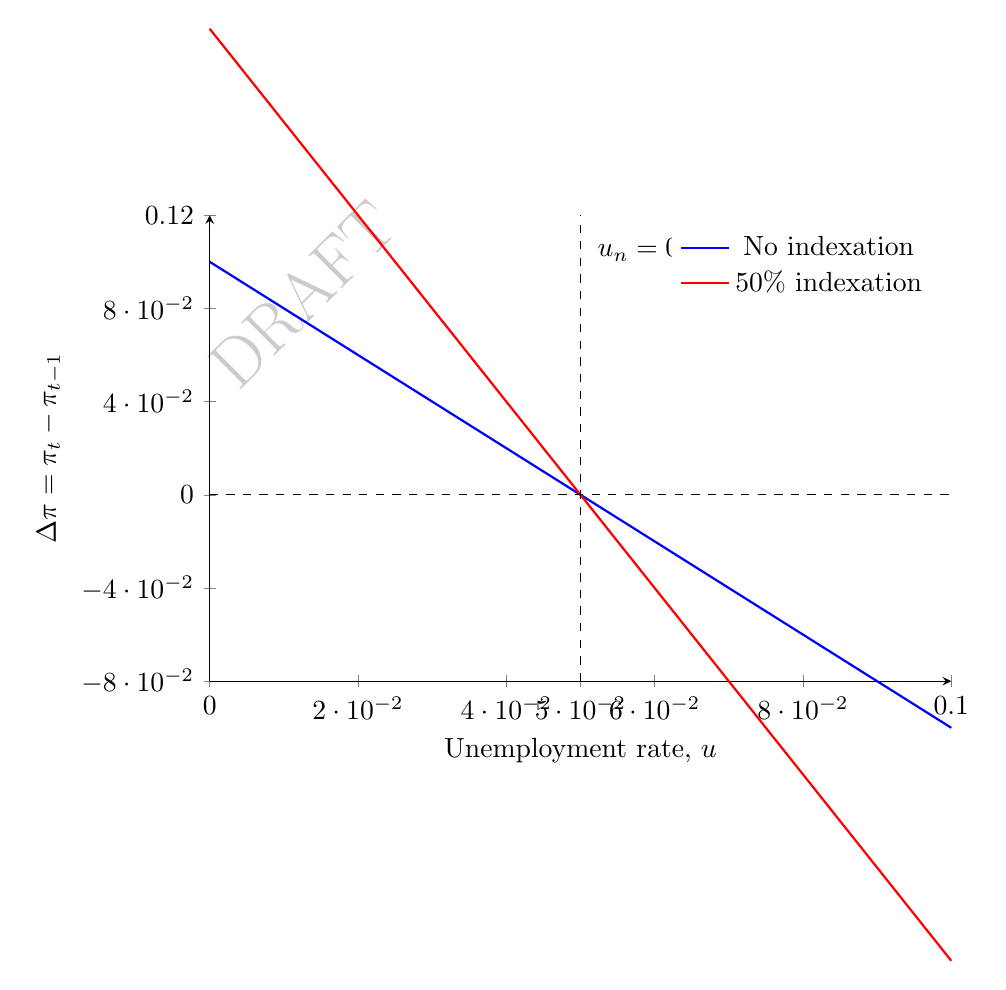
\begin{tikzpicture}
\begin{axis}[
    width=11cm,
    height=7.5cm,
    xmin=0,
    xmax=0.1,
    ymin=-0.08,
    ymax=0.12,
    axis lines=left,
    xlabel={Unemployment rate, \(u\)},
    ylabel={\(\Delta \pi = \pi_t-\pi_{t-1}\)},
    xtick={0,0.02,0.04,0.05,0.06,0.08,0.1},
    ytick={-0.08,-0.04,0,0.04,0.08,0.12},
    legend style={draw=none, at={(0.98,0.98)}, anchor=north east},
    clip=false
]
\addplot[domain=0:0.1,samples=2,thick,blue] {0.1 - 2*x};
\addplot[domain=0:0.1,samples=2,thick,red] {0.2 - 4*x};
\addplot[dashed] coordinates {(0.05,-0.08) (0.05,0.12)};
\addplot[dashed] coordinates {(0,0) (0.1,0)};
\legend{No indexation, 50\% indexation}
\node[anchor=west] at (axis cs:0.051,0.105) {\(u_n=0.05\)};
\end{axis}
\end{tikzpicture}
\end{center}

\end{document}
